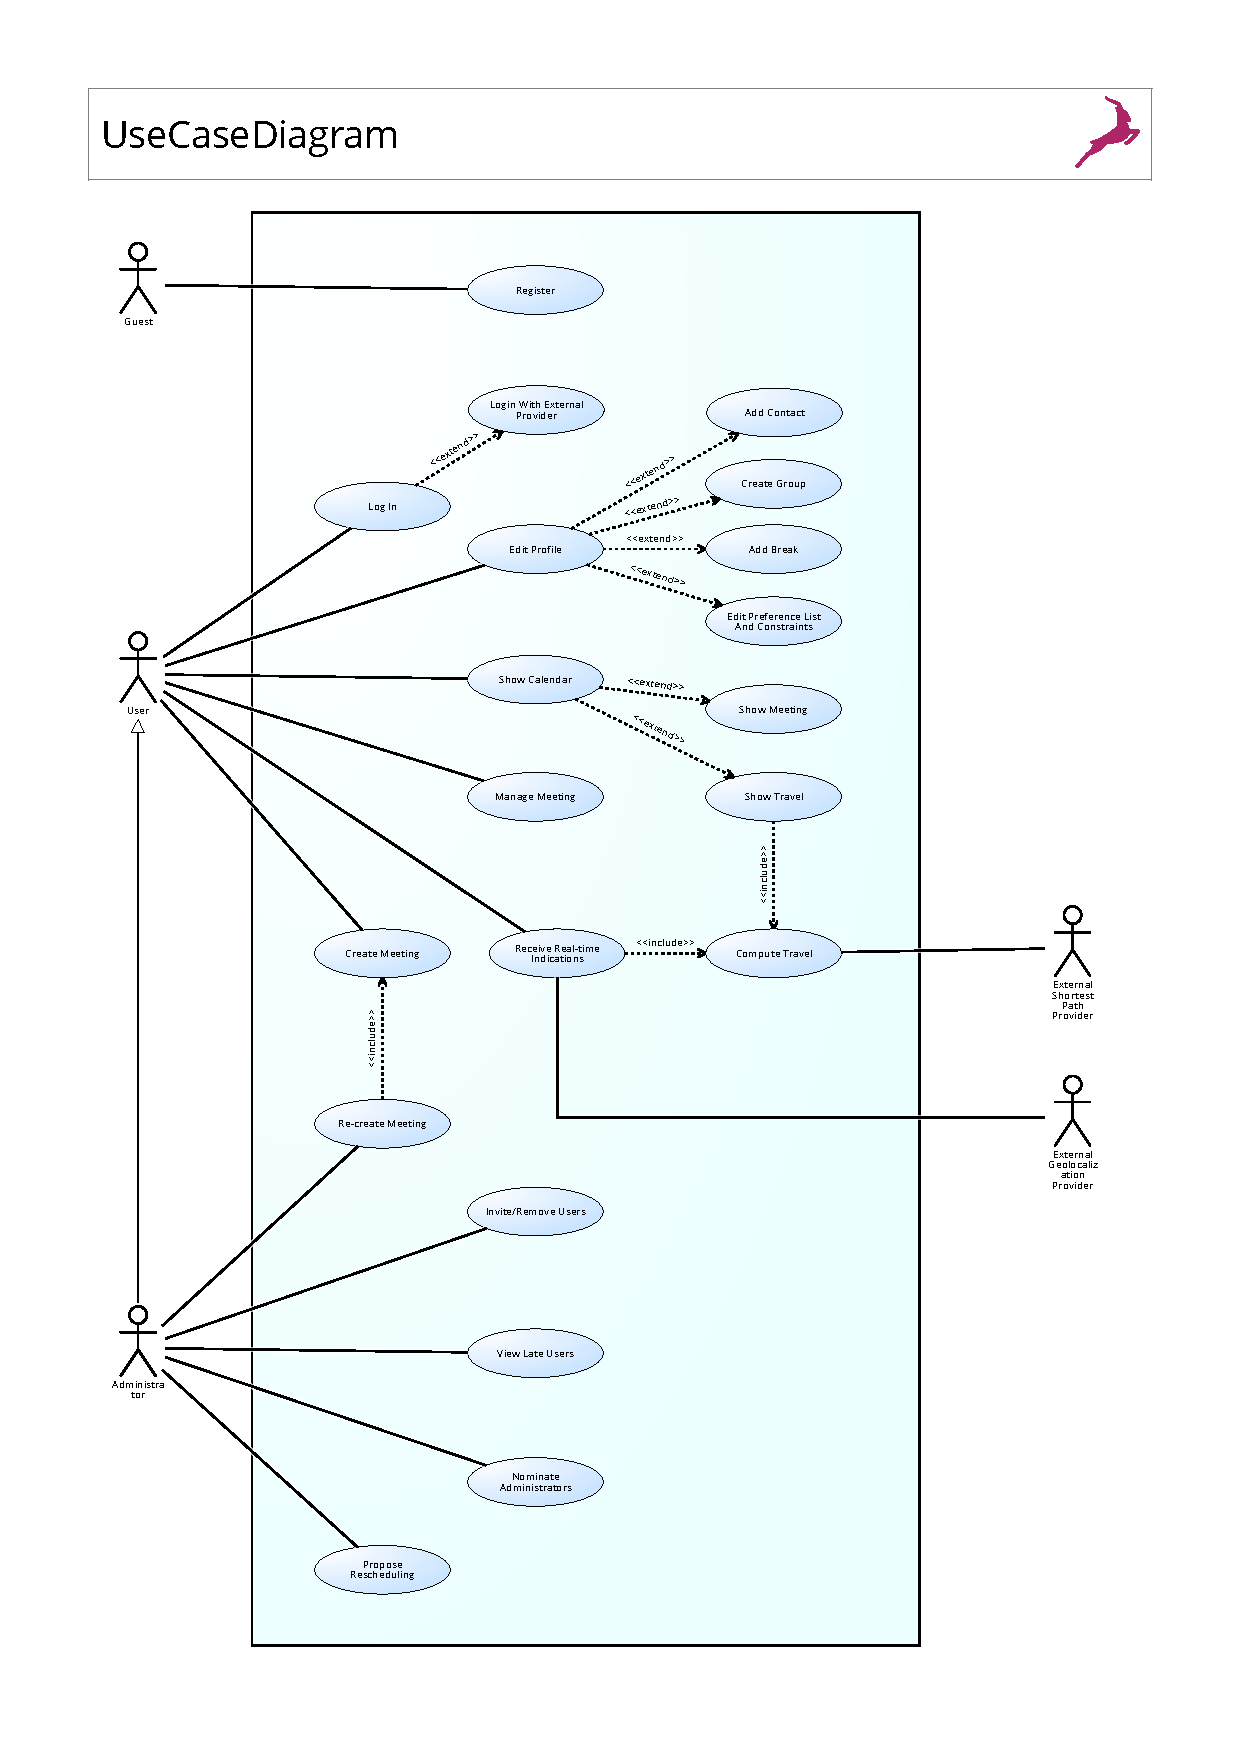
\includepdf[pages=-]{Pdf/UseCaseDiagram.pdf}

\begin{table}[H]
	\centering
	\def\arraystretch{1.5}
	\begin{tabular}{|p{7cm}|p{7cm}|}
		\hline
		\textbf{Actors}            & Guest		    \\ \hline
		\textbf{Goals}             &            \\ \hline
		\textbf{Input Conditions}  &            \\ \hline
		\textbf{Events Flow}       &            \\ \hline
		\textbf{Output Conditions} &            \\ \hline
		\textbf{Exceptions}        &            \\ \hline
	\end{tabular}
	\caption{Register}
\end{table}

\begin{table}[H]
	\centering
	\def\arraystretch{1.5}
	\begin{tabular}{|p{7cm}|p{7cm}|}
		\hline
		\textbf{Actors}            & User, External Login Provider		    \\ \hline
		\textbf{Goals}             & G2           \\ \hline
		\textbf{Input Conditions}  & User is on the homepage of the system and it has not yet been authenticated.           \\ \hline
		\textbf{Events Flow}       &    
		 	Login via user credentials
			 	\begin{enumerate}
			 		\item The user inserts its main email address or its nickname
			 		\item The user inserts its password
			 		\item The user clicks on the "Log in" button and is authenticated
			 	\end{enumerate}
		 	Login via External Service Provider
			 	\begin{enumerate}
				 	\item The user clicks on the "Log in with \texttt{Service name}" button
				 	\item The user is taken to an external page where it has to follow the authentication procedure of the external login provider
				 	\item The user is redirected to our system with a valid token
			 	\end{enumerate} \\ \hline
		\textbf{Output Conditions} & User is logged into the system.          \\ \hline
		\textbf{Exceptions}        & The user credentials are wrong or the external login provider procedure cannot be completed correctly. In either case the system shows the user a message reporting the errors and waits for another attempt.         \\ \hline
	\end{tabular}
	\caption{Login}
\end{table}

\begin{table}[H]
	\centering
	\def\arraystretch{1.5}
	\begin{tabular}{|p{7cm}|p{7cm}|}
		\hline
		\textbf{Actors}            & User		    \\ \hline
		\textbf{Goals}             & G3           \\ \hline
		\textbf{Input Conditions}  & The user has already been authenticated by the system.           \\ \hline
		\textbf{Events Flow}       & 
			\begin{enumerate}[topsep=0pt, leftmargin=*]
				\item The user selects a field in its profile
				\item The user inserts new data for the selected field
				\item The user can repeat from point 1 or click the "Save" button
			\end{enumerate}           \\ \hline
		\textbf{Output Conditions} & The selected fields are updated with the new data inserted by the user.          \\ \hline
		\textbf{Exceptions}        &  The data inserted in a field are wrong (e.g. a non-unique nickname, a non-unique email, a syntactically wrong website). The system shows the user a message reporting the errors, clears the incorrect fields and restart the event flow from point 1.               \\ \hline
	\end{tabular}
	\caption{Edit Profile}
\end{table}

\begin{table}[H]
	\centering
	\def\arraystretch{1.5}
	\begin{tabular}{|p{7cm}|p{7cm}|}
		\hline
		\textbf{Actors}            & User		    \\ \hline
		\textbf{Goals}             &            \\ \hline
		\textbf{Input Conditions}  &            \\ \hline
		\textbf{Events Flow}       &            \\ \hline
		\textbf{Output Conditions} &            \\ \hline
		\textbf{Exceptions}        &            \\ \hline
	\end{tabular}
	\caption{Show Calendar}
\end{table}

\begin{table}[H]
	\centering
	\def\arraystretch{1.5}
	\begin{tabular}{|p{7cm}|p{7cm}|}
		\hline
		\textbf{Actors}            & User		    \\ \hline
		\textbf{Goals}             &            \\ \hline
		\textbf{Input Conditions}  &            \\ \hline
		\textbf{Events Flow}       &            \\ \hline
		\textbf{Output Conditions} &            \\ \hline
		\textbf{Exceptions}        &            \\ \hline
	\end{tabular}
	\caption{Manage Meetings}
\end{table}

\begin{table}[H]
	\centering
	\def\arraystretch{1.5}
	\begin{tabular}{|p{7cm}|p{7cm}|}
		\hline
		\textbf{Actors}            & User, External Geolocalization Provider		    \\ \hline
		\textbf{Goals}             &            \\ \hline
		\textbf{Input Conditions}  &            \\ \hline
		\textbf{Events Flow}       & 	        \\ \hline
		\textbf{Output Conditions} &            \\ \hline
		\textbf{Exceptions}        &            \\ \hline
	\end{tabular}
	\caption{Receive Real-Time Indications}
\end{table}

\begin{table}[H]
	\centering
	\def\arraystretch{1.5}
	\begin{tabular}{|p{7cm}|p{7cm}|}
		\hline
		\textbf{Actors}            & User		    \\ \hline
		\textbf{Goals}             & G4           \\ \hline
		\textbf{Input Conditions}  & The user has already been authenticated by the system.           \\ \hline
		\textbf{Events Flow}       & 
			\begin{enumerate}[topsep=0pt, leftmargin=*]
				\item The user inserts a start date, an end date, a title and a location for the meeting
				\item The user may add other data, such as an abstract or a category
				\item The user chooses a non-empty list of invited users, either by inserting their email or by selecting them from its contacts; in alternative the user may specify that it is an instant meeting
				\item The user clicks on the "Create" button
			\end{enumerate}               \\ \hline
		\textbf{Output Conditions} & A new meeting is created and an invitation is sent to all the selected users.           \\ \hline
		\textbf{Exceptions}        & The location of the meeting may be incorrect or the start and end date may be inconsistent (i.e. the start is after the end). The system shows the user a message reporting the errors, clears the incorrect fields and restart the event flow from point 1.          \\ \hline
	\end{tabular}
	\caption{Create Meeting}
\end{table}

\begin{table}[H]
	\centering
	\def\arraystretch{1.5}
	\begin{tabular}{|p{7cm}|p{7cm}|}
		\hline
		\textbf{Actors}            & Administrator    \\ \hline
		\textbf{Goals}             & G4           \\ \hline
		\textbf{Input Conditions}  & Un meeting è stato creato ed effettuato normalmente.           \\ \hline
		\textbf{Events Flow}       &            \\ \hline
		\textbf{Output Conditions} & Il sistema invia un invito ai parteciapnti, che devono decidere se accettare, declinnare o rischedulare, del nuovo meeting            \\ \hline
		\textbf{Exceptions}        &            \\ \hline
	\end{tabular}
	\caption{Recreate Meeting}
\end{table}

\begin{table}[H]
	\centering
	\def\arraystretch{1.5}
	\begin{tabular}{|p{7cm}|p{7cm}|}
		\hline
		\textbf{Actors}            & Administrator    \\ \hline
		\textbf{Goals}             &            \\ \hline
		\textbf{Input Conditions}  &            \\ \hline
		\textbf{Events Flow}       &            \\ \hline
		\textbf{Output Conditions} &            \\ \hline
		\textbf{Exceptions}        &            \\ \hline
	\end{tabular}
	\caption{Invite/Remove Users}
\end{table}

\begin{table}[H]
	\centering
	\def\arraystretch{1.5}
	\begin{tabular}{|p{7cm}|p{7cm}|}
		\hline
		\textbf{Actors}            & Administrator    \\ \hline
		\textbf{Goals}             &            \\ \hline
		\textbf{Input Conditions}  &            \\ \hline
		\textbf{Events Flow}       &            \\ \hline
		\textbf{Output Conditions} &            \\ \hline
		\textbf{Exceptions}        &            \\ \hline
	\end{tabular}
	\caption{View Late Users}
\end{table}

\begin{table}[H]
	\centering
	\def\arraystretch{1.5}
	\begin{tabular}{|p{7cm}|p{7cm}|}
		\hline
		\textbf{Actors}            & Administrator    \\ \hline
		\textbf{Goals}             &            \\ \hline
		\textbf{Input Conditions}  &            \\ \hline
		\textbf{Events Flow}       &            \\ \hline
		\textbf{Output Conditions} &            \\ \hline
		\textbf{Exceptions}        &            \\ \hline
	\end{tabular}
	\caption{Nominate Administrators}
\end{table}

\begin{table}[H]
	\centering
	\def\arraystretch{1.5}
	\begin{tabular}{|p{7cm}|p{7cm}|}
		\hline
		\textbf{Actors}            & Administrator    \\ \hline
		\textbf{Goals}             &            \\ \hline
		\textbf{Input Conditions}  &            \\ \hline
		\textbf{Events Flow}       &            \\ \hline
		\textbf{Output Conditions} &            \\ \hline
		\textbf{Exceptions}        &            \\ \hline
	\end{tabular}
	\caption{Propose Rescheduling}
\end{table}